\subsection{Propriedades do Clock}

Formalmente, um sinal de clock pode ser modelado como uma função periódica discreta ou contínua no tempo. No contexto físico, considera-se inicialmente uma representação contínua:

\[
clk : \mathbb{R}_{\geq 0} \to \{0,1\}
\]

tal que:

\[
clk(t + T) = clk(t)
\]

onde \(T > 0\) representa o período do sinal.

A frequência do clock é definida como o inverso do período:

\[
f = \frac{1}{T}
\]

Em sistemas digitais síncronos, o clock estabelece os instantes nos quais os elementos de memória amostram suas entradas e atualizam seus estados internos. Dessa forma, embora o sinal físico exista continuamente no tempo, a evolução lógica do sistema ocorre apenas em instantes discretos:

\[
t_n = nT, \quad n \in \mathbb{N}
\]


Assim, o período \(T\) pode ser decomposto em dois intervalos:

\[
T = t_{high} + t_{low}
\]

onde:

\begin{itemize}
    \item \(t_{high}\): duração do nível lógico alto;
    \item \(t_{low}\): duração do nível lógico baixo.
\end{itemize}

A razão entre o tempo em nível alto e o período total define o \textit{duty cycle} $D$ do sinal:

\[
D = \frac{t_{high}}{T}
\]

Esse parâmetro é relevante em circuitos sensíveis à largura temporal dos pulsos.

\begin{figure}[H]
    \centering
    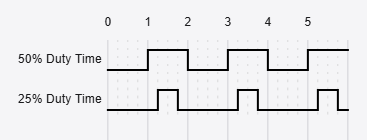
\includegraphics[width=0.7\linewidth]{images/duty-cycles.png}
    \caption{Exemplos de duty cycle}
    \label{fig:duty-cycles}
\end{figure}

Além disso, sendo um sinal periódico, o clock pode ser descrito por uma fase instantânea \(\theta(t)\), que representa sua posição relativa dentro de um ciclo.

Matematicamente:

\[
\theta(t) = 2\pi \frac{t \bmod T}{T}
\]

com:

\[
\theta(t) \in [0, 2\pi)
\]

A fase fornece uma representação contínua da evolução temporal do sinal ao longo de um período.

Embora sistemas digitais normalmente não utilizem diretamente o valor contínuo da fase, eventos específicos associados a ela possuem importância fundamental. Em particular:

\begin{itemize}
    \item \(\theta = 0\): borda de subida;
    \item \(\theta = \pi\): borda de descida.
\end{itemize}

Essas transições definem os instantes nos quais máquinas de estado e elementos sequenciais realizam atualizações sincronizadas.

A modelagem em termos de fase também é útil para a análise de fenômenos temporais como:

\begin{itemize}
    \item \textit{skew}: desalinhamento temporal do clock entre diferentes regiões do circuito;
    \item \textit{jitter}: variações temporais na periodicidade do sinal.
\end{itemize}

Assim, um sinal de clock periódico pode ser caracterizado de forma compacta, pela tupla de parâmetros:

\[
(T, D, \theta_0)
\]